\documentclass[crop, tikz]{standalone}
\usepackage{tikz}

\usetikzlibrary{positioning}

\tikzstyle{stateTransition}=[-stealth, thick]

\begin{document}
\begin{tikzpicture}
	
	\node[rectangle, draw, minimum width=0.5cm,minimum height=2.5cm] (X) at (-2, 0) {$\vec{x}$};
	
	\node[rectangle, draw, right=1.5em of X, text depth=0em, minimum width=1.5cm,minimum height=2.5cm] (W1) {${\bf W_1}\times$};

	\node[rectangle, draw, right=1.5em of W1, text depth=0em, minimum width=0.5cm,minimum height=2.5cm] (B1) {$+ \vec{b}_1$};
	
	\node[rectangle, draw, right=1.5em of B1, text depth=0em, minimum width=1.5cm,minimum height=2.5cm] (RL) {
		\begin{tikzpicture}
			\draw[thick] (0,0) -- (0.5, 0);
			\draw[thick] (0.49,-0.004) -- (0.99, 0.496);
		\end{tikzpicture}
	};
	
	\node[rectangle, draw, right=1.5em of RL, text depth=0em, minimum width=1.5cm,minimum height=2.5cm] (W) {${\bf W_2}\times$};

	\node[rectangle, draw, right=1.5em of W, text depth=0em, minimum width=0.5cm,minimum height=1.5cm] (B) {$+ \vec{b}_2$};
	
	\node[right=1.5em of B, inner sep=0em] (out) {
	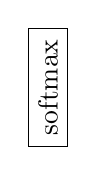
\begin{tikzpicture}
		\node[rectangle, draw, rotate=90, minimum height=0.5cm, minimum width=1.5cm] (out) {softmax};
	\end{tikzpicture}
	};
	
	\node[right=1.5em of out] (outt) {};
	
	\foreach \x in {1,...,3}
    		\draw[stateTransition] ([yshift=\x em]X.east) -- ([yshift=\x em]W1.west);
    \foreach \x in {1,...,3}
    		\draw[stateTransition] ([yshift=-\x em]X.east) -- ([yshift=-\x em]W1.west);
	\draw[-stealth, thick] (X) -- (W1);
	
	\foreach \x in {1,...,3}
    		\draw[stateTransition] ([yshift=\x em]W1.east) -- ([yshift=\x em]B1.west);
    \foreach \x in {1,...,3}
    		\draw[stateTransition] ([yshift=-\x em]W1.east) -- ([yshift=-\x em]B1.west);
	\draw[-stealth, thick] (W1) -- (B1);
	
	\foreach \x in {1,...,3}
    		\draw[stateTransition] ([yshift=\x em]B1.east) -- ([yshift=\x em]RL.west);
    \foreach \x in {1,...,3}
    		\draw[stateTransition] ([yshift=-\x em]B1.east) -- ([yshift=-\x em]RL.west);
	\draw[-stealth, thick] (B1) -- (RL);
	
	\foreach \x in {1,...,3}
    		\draw[stateTransition] ([yshift=\x em]RL.east) -- ([yshift=\x em]W.west);
    \foreach \x in {1,...,3}
    		\draw[stateTransition] ([yshift=-\x em]RL.east) -- ([yshift=-\x em]W.west);
	\draw[-stealth, thick] (RL) -- (W);
	
	\foreach \x in {-1.5, -0.5, 0.5, 1.5}
    		\draw[stateTransition] ([yshift=\x em]W.east) -- ([yshift=\x em]B.west);
	\foreach \x in {-1.5, -0.5, 0.5, 1.5}
    		\draw[stateTransition] ([yshift=\x em]B.east) -- ([yshift=\x em]out.west);
	\foreach \x in {-1.5, -0.5, 0.5, 1.5}
    		\draw[stateTransition] ([yshift=\x em]out.east) -- ([yshift=\x em]outt.west);
	
\end{tikzpicture}
\end{document}